\begin{frame}{Orthogonal sets}
\begin{definition}
Let $(V,\langle \ , \rangle)$ be an inner product space. 

A set $S=\{\boldv_1,\boldv_2,\dots,\boldv_r\}$ of {\em nonzero vectors} is {\bf orthogonal} if $\langle\boldv_i,\boldv_j\rangle=0$ for all $i\ne j$: i.e., the elements are pairwise orthogonal. 

An orthogonal set that further satisfies $\norm{\boldv_i}=1$ for all $i$ is called {\bf orthonormal}.   
\end{definition}
\pause
\begin{theorem}
Let $(V,\langle\ , \rangle)$ be an inner product space. If $S=\{\boldv_1,\boldv_2,\dots,\boldv_r\}$ is orthogonal, then $S$ is linearly independent. 
\end{theorem}
\pause
\begin{proof}
\begin{eqnarray*}
a_1\boldv_1 +a_2\boldv_2+\cdots +a_r\boldv_r=\boldzero&\Rightarrow& \langle a_1\boldv_1 +a_2\boldv_2 +\cdots +a_r\boldv_r,\boldv_i\rangle=\langle\boldzero,\boldv_i\rangle \\
\pause&\Rightarrow& a_1\langle\boldv_1,\boldv_i\rangle +a_2\langle \boldv_2,\boldv_i\rangle +\cdots +a_r\langle\boldv_r,\boldv_i\rangle=0 \\
\pause&\Rightarrow& a_i\langle \boldv_i,\boldv_i\rangle=0 \ \text{ (since $\langle\boldv_j,\boldv_i\rangle= 0$ for $j\ne i$)}\\
\pause&\Rightarrow& a_i=0  \text{ (since $\langle\boldv_i,\boldv_i\rangle\ne 0$)}
\end{eqnarray*}
We have shown that if $a_1\boldv_1+a_2\boldv_2+\cdots +a_r\boldv_r=\boldzero$, then $a_i=0$ for all $i$, proving that $S$ is linearly independent. 
\end{proof}
\end{frame}
\begin{frame}{Example}
Let $V=C([0,2\pi])$ with standard inner product $\langle f, g\rangle=\int_0^{2\pi} f(x)g(x) \, dx$. 

Let \[ S=\{\cos(x),\sin(x),\cos(2x),\sin(2x), \dots\}=\{\cos(nx)\colon n\in\Z_{>0}\}\cup\{\sin(mx)\colon m\in\Z_{>0}\}.\] Then $S$ is orthogonal, hence linearly independent. 
\pause
\begin{proof}
Using some trig identities, one can show the following:
\begin{align*}
\langle \cos(nx),\cos(mx)\rangle=\int_0^{2\pi}\cos(nx)\cos(mx)\, dx&=\begin{cases} 0& \text{ if $n\ne m$} \\ \pi& \text{ if $n=m$} \end{cases}\\
\langle \sin(nx),\sin(mx)\rangle=\int_0^{2\pi}\sin(nx)\sin(mx)\, dx&=\begin{cases} 0& \text{ if $n\ne m$} \\ \pi& \text{ if $n=m$} \end{cases}\\
\langle \cos(nx),\sin(mx)\rangle=\int_0^{2\pi}\cos(nx)\sin(mx)\, dx&=0 \text{ for any $n,m$}
\end{align*}
\end{proof}
\pause Orthogonality holds more generally if we replace the interval $[0,2\pi]$ with any interval of length $L$, and replace $S$ with 
\[\scriptsize
\left\{\cos\left(\frac{2\pi x}{L}\right), \sin\left(\frac{2\pi x}{L}\right), \cos\left(2\cdot\frac{2\pi x}{L}\right),\sin\left(2\cdot\frac{2\pi x}{L}\right),\dots\right\}.
\]

\end{frame}
\begin{frame}{Orthogonal basis}
\begin{definition}
Let $(V,\langle \ , \rangle)$ be an inner product space, $\dim V=n$. 

An {\bf orthogonal basis} is a basis $B=\{\boldv_1,\dots,\boldv_n\}$ that is an orthogonal set; an orthogonal basis $B$ is {\bf orthonormal} if $B$ is orthonormal.     
\end{definition}
\pause
\begin{theorem}[Existence/extension of orthonormal bases]
Let $(V,\langle \ , \rangle)$ be a finite-dimensional inner product vector space. 

Then \alert{(1)} $V$ has an ortho(gonal/normal) basis. (Proof is the \alert{Gram-Schmidt} process. See two slides on.) 

Furthermore, \alert{(2)} any ortho(gonal/normal) set can be \alert{extended} to an ortho(gonal/normal) basis of $V$. 
 \end{theorem}
\end{frame}
\begin{frame}
\begin{theorem}[Calculating with ortho(gonal/normal) bases]
Let $B=\{\boldv_1,\dots,\boldv_n\}$ be an \alert{orthogonal basis} for $V$. 

Given any $\boldv\in V$ we have $\boldv=a_1\boldv_1+a_2\boldb_2+\cdots +a_n\boldv_n$ where 
$
a_i=\frac{\langle \boldv,\boldv_i\rangle}{\langle\boldv_i,\boldv_i\rangle}.
$
 
\pause Equivalently, 
\[
[\boldv]_B=\begin{bmatrix}
\frac{\langle \boldv,\boldv_1\rangle}{\langle\boldv_1,\boldv_1\rangle}\\
\frac{\langle \boldv,\boldv_2\rangle}{\langle\boldv_2,\boldv_2\rangle}\\
\vdots \\
\frac{\langle \boldv,\boldv_n\rangle}{\langle\boldv_n,\boldv_n\rangle}
\end{bmatrix}
\]
\pause If $B$ is ortho\alert{normal} then these formulas simplify to 
\[
a_i=\langle\boldv,\boldv_i\rangle \text{ for all $i$}.
\] 
\end{theorem}
\end{frame}

\begin{frame}{Example}
Let $V=\R^2$ with the standard inner produce (aka the dot product). 

(a) Verify that $B'=\{\boldv_1=(\sqrt{3}/2,1/2), \boldv_2=(-1/2,\sqrt{3}/2)\}$ is an orthonormal basis. 

(b) Compute $[\boldv]_{B'}$ for $\boldv=(4,2)$. 

(c) Compute $\underset{B\rightarrow B'}{P}$, where $B$ is the standard basis. 
\begin{bsolution}
\ \\
(a) Easily seen to be true. 

(b) Since $B'$ is orthonormal, $\boldv=a_1\boldv_1+a_2\boldv_2$ where $a_1=\boldv\cdot\boldv_1=2\sqrt{3}+1$ and $a_2=\boldv\cdot\boldv_2=\sqrt{3}-2$. Thus $[\boldv]_{B'}=\begin{bmatrix}
2\sqrt{3}+1\\
\sqrt{3}-2
\end{bmatrix}
$

\pause
(c) As we have seen before, $\underset{B'\rightarrow B}{P}=\begin{bmatrix}[rr]
\sqrt{3}/2&-1/2\\1/2&\sqrt{3}/2
\end{bmatrix}$ (put elements of $B'$ in as columns). Hence $\underset{B\rightarrow B'}{P}=(\underset{B'\rightarrow B}{P})^{-1}=\begin{bmatrix}[rr]
\sqrt{3}/2&1/2\\-1/2&\sqrt{3}/2
\end{bmatrix}
$
\end{bsolution}

\pause\alert{Useful fact}. If the columns of an $n\times n$ matrix $P$ are orthonormal, then $P$ is invertible, and $\boxed{P^{-1}=P^T}$. 
\bpause
\alert{Proof}. Let $\boldp_j$ be the $j$-th column of $P$. By the \alert{dot product method} of matrix multiplication, we have 
$P^TP=[\boldp_i\cdot\boldp_j]=I_n$, since the $\boldp_i$ are orthonormal. This proves $P^T=P^{-1}$. 
\end{frame}
\begin{frame}{Gram-Schmidt Process}
The proof that every finite-dimensional vector space has an orthogonal basis is actually a procedure, called the \alert{Gram-Schmidt process}, for converting an arbitrary basis for an inner product space to an orthogonal basis.
\pause
\begin{theorem}[Gram-Schmidt process]
Let $(V, \langle \ , \ \rangle)$ be an inner product space, and let $B=\{\boldv_1, \boldv_2, \dots, \boldv_n\}$ be a basis for $V$. We can convert $B$ into an orthogonal basis $B'=\{\boldw_1, \boldw_2, \dots, \boldw_n\}$ using the following recursive procedure: 
\bb
\ii Set $\boldw_1=\boldv_1$. 
\ii For $2\leq r\leq n$ replace $\boldv_r$ with 
\[
\boldw_r:=\boldv_r-\frac{\angvec{\boldv_r, \boldw_{r-1}}}{\angvec{\boldw_{r-1},\boldw_{r-1}}}\boldw_{r-1}-\frac{\angvec{\boldv_r, \boldw_{r-2}}}{\angvec{\boldw_{r-2},\boldw_{r-2}}}\boldw_{r-2}-\cdots -\frac{\angvec{\boldv_r, \boldw_{1}}}{\angvec{\boldw_{1},\boldw_{1}}}\boldw_1
\]
\ee
Lastly, to further transform to an orthonormal basis, replace each $\boldw_i$ with $\ds \boldu_i=\frac{\boldw_i}{\norm{\boldw_i}}$. 
\end{theorem}
\end{frame}
\begin{frame}{Orthogonal complement}
\begin{definition}. 
 Let $(V,\langle \ , \rangle)$ be an inner product vector space, and let $W\subseteq V$ be a finite-dimensional subspace. 
 The {\bf orthogonal complement of $W$} is defined as 
\[
W^\perp:=\{\boldv\in V\colon \langle \boldv, \boldw\rangle=0 \text{ for all }\boldw\in W\}.
\]
In English: $W^\perp$ is the set of vectors that are orthogonal to {\em all} vectors in $W$. 
\end{definition}
\pause
\begin{theorem}[Orthogonal complement theorem]
Let $(V,\langle \ , \rangle)$ be an inner product vector space, and let $W\subseteq V$ be a subspace. 
\bb[(a)]
\ii $W^\perp$ is a subspace of $V$. 
\ii $W\cap W^\perp=\{\boldzero\}$
\ee
\end{theorem}
\pause 
\alert{Example}. Let $V=\R^3$ equipped with the dot product, and let $W=\Span\{(1,1,1)\}\subset \R^3$. This is the line defined by the vector $(1,1,1)$. Then $W^\perp$ is the set of vectors orthogonal to $(1,1,1)$: i.e., the plane perpendicular to $(1,1,1)$. 
\end{frame}

\begin{frame}{Geometry of fundamental spaces}
The notion of orthogonal complement gives us a new way of understanding the relationship between the various fundamental spaces of a matrix. 
\pause
\begin{theorem}
Let $A$ be $m\times n$, and consider $\R^n$ and $\R^m$ as inner product spaces with respect to the dot product. Then:
\bb[(i)]
\ii $\NS(A)=\left(\RS(A)\right)^\perp$, and thus $\RS(A)=\left(\NS(A)\right)^\perp$.
\ii $\NS(A^T)=\left(\CS(A)\right)^\perp$, and thus $\CS(A)=\left(\NS(A^T)\right)^\perp$.
\ee
\end{theorem}
\pause
\begin{proof}
\ \\
(i) Using the dot product method of matrix multiplication, we see that a vector $\boldv\in\NS(A)$ if and only if $\boldv\cdot\boldr_i=0$ for each row $\boldr_i$ of $A$. Since the $\boldr_i$ span $\RS(A)$, the linear properties of the dot product imply that $\boldv\cdot\boldr_i=0$ for each row $\boldr_i$ of $A$ if and only if $\boldv\cdot\boldw=0$ for \alert{all} $\boldw\in\RS(A)$ if and only if $\boldv\in \RS(A)^\perp$. 
\bpause
(ii) This follows from (i) and the fact that $\CS(A)=\RS(A^T)$. 

\end{proof}
\end{frame}
\begin{frame}{Visualizing the rank-nullity theorem}
\[
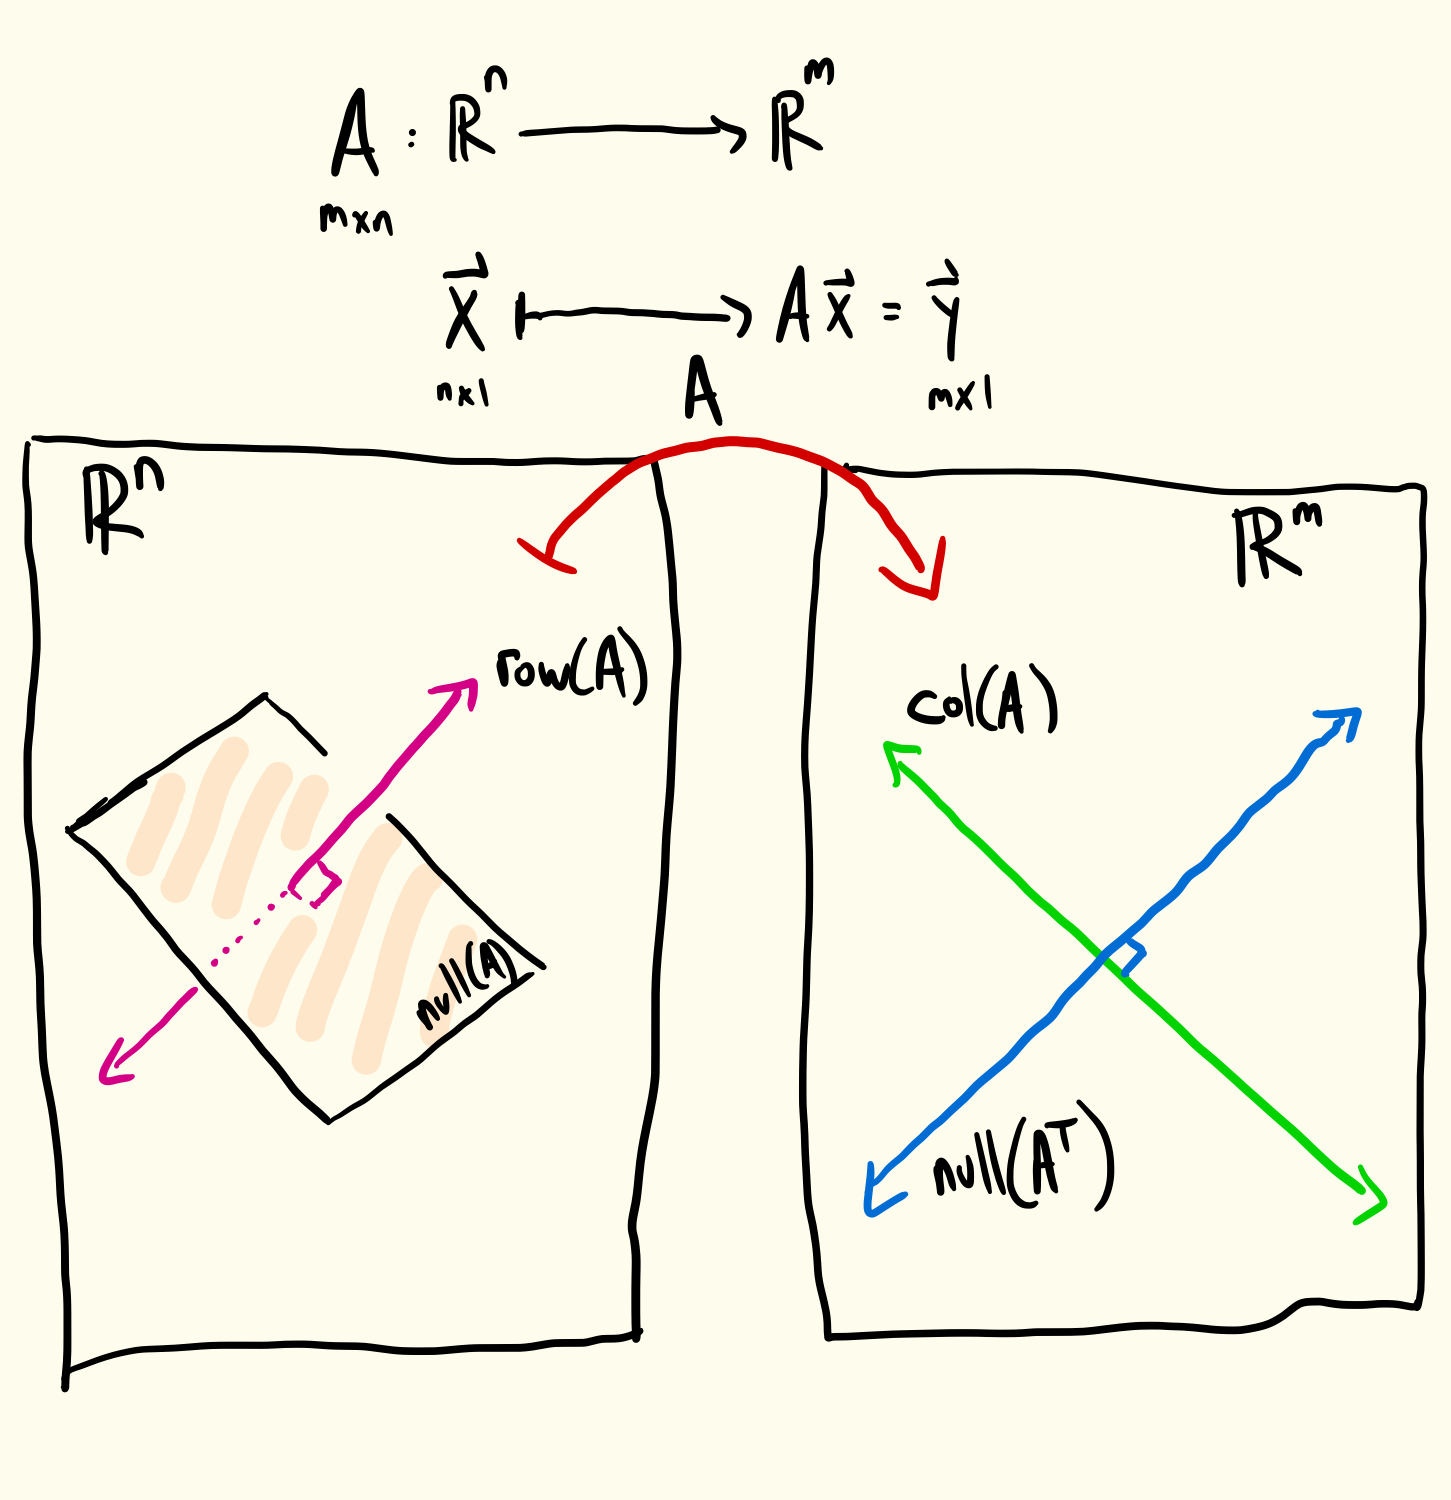
\includegraphics[width=3.5in]{Images/RankNullity}
\]
\end{frame}
\begin{frame}{Example}
Understanding the orthogonal relationship between $\NS(A)$ and $\RS(A)$ allows us in many cases to quickly determine/visualize the one from the other. 
\bspace
Consider the example $A=\begin{bmatrix}[rrr]
1&-1&1\\
1&-1&-1
\end{bmatrix}
$.
\pause Looking at the columns, we see easily that $\rank(A)=2$, which implies that $\nullity(A)=3-2=1$. Since $(1,-1,0)$ is an element of $\NS(A)$ and $\dim(\NS(A))=1$, we must have $\NS(A)=\Span\{(1,-1,0)\}$, a line. 
\bpause
By orthogonality, we conclude that 
\[ \RS(A)=\NS(A)^\perp=\text{(plane perpendicular to $(1,-1,0)$)}. 
\]
\[
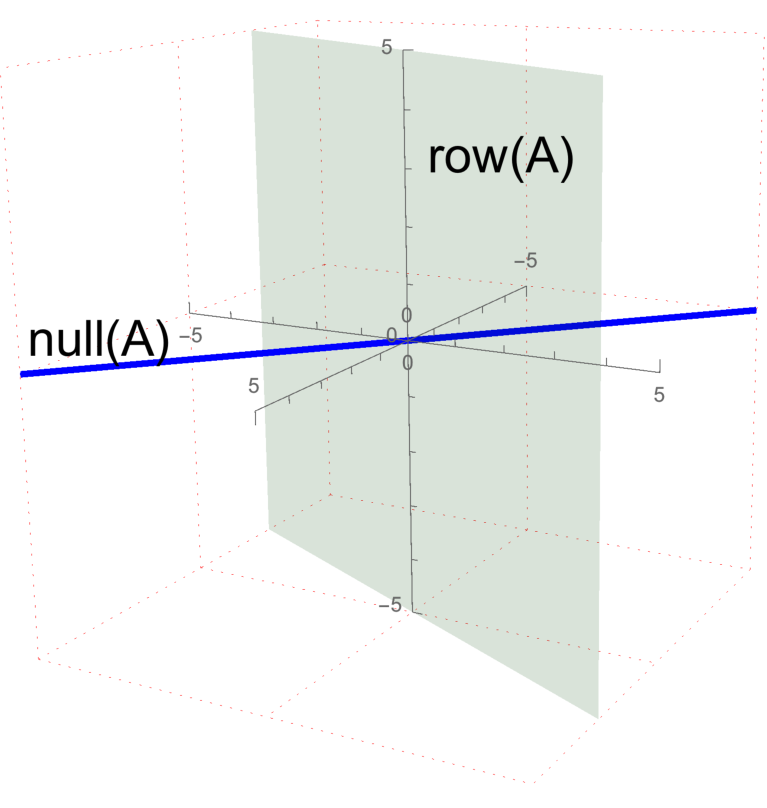
\includegraphics[width=2in]{Images/NullRow}
\]
\end{frame}
\begin{frame}{Orthogonal Projection}
\begin{theorem}[Orthogonal projection theorem]
Let $(V,\langle \ , \rangle)$ be an inner product space, and let $W\subseteq V$ be a \alert{finite-dimensional} subspace. 
\bb[(a)]
\ii (Orthogonal decomposition). 
For all $\boldv\in V$ there is a unique choice of vectors $\boldw\in W$ and $\boldw^\perp\in W^\perp$ such that $\boldv=\boldw+\boldw^\perp$. 

We call this vector expression an {\bf orthogonal decomposition} of $\boldv$, and denote $\boldw=\proj{\boldv}{W}$ and $\boldw^\perp=\proj{\boldv}{W^\perp}$, the {\bf orthogonal projections} of $\boldv$ onto $W$ and $W^\perp$, respectively. 
\pause\ii The orthogonal projection $\boldw=\proj{\boldv}{W}$ is the element of $W$ \alert{closest} to $\boldv$. This means $\norm{\boldv-\proj{\boldv}{W}}\leq\norm{\boldv-\boldw'}$ for any other $\boldw'\in W$. We thus define the distance from $\boldv$ to $W$ as $d(\boldv, W)=\norm{\boldv-\proj{\boldv}{W}}=\norm{\boldw^\perp}$. 
\pause\ii (Orthogonal projection formula). Pick an {\em orthogonal} basis $B=\{\boldv_1,\boldv_2,\dots, \boldv_r\}$ of $W$. 
Then $\ds \proj{\boldv}{W}=\sum_{i=1}^r\frac{\angvec{\boldv,\boldv_i}}{\angvec{\boldv_i, \boldv_i}}\boldv_i$.
\ee
\pause
\begin{comment}
An important consequence of this theorem is that $\proj{\boldv}{W}$ can be uniquely characterized by two distinct properties:

(i) it is the unique element $\boldw$ of $W$ \alert{closest} to $\boldv$

(ii) it is the unique element $\boldw$ of $W$ such that $\boldv-\boldw$ is \alert{orthogonal} to $W$. 
\end{comment}
\end{theorem}
\end{frame}
\begin{frame}{Proof of orthogonal projection theorem}\scriptsize
Pick an {\em orthogonal} basis $B=\{\boldv_1,\boldv_2,\dots, \boldv_r\}$ of $W$ and set $\boldw=\sum_{i=1}^r\frac{\angvec{\boldv,\boldv_i}}{\angvec{\boldv_i, \boldv_i}}\boldv_i$. This is clearly an element of $W$. Next we set $\boldw^\perp=\boldv-\boldw=\boldv-\sum_{i=1}^r\frac{\angvec{\boldv,\boldv_i}}{\angvec{\boldv_i, \boldv_i}}\boldv_i$. 
\bpause
To complete the proof, we must show the following: (A) $\boldw^\perp\in W^\perp$, (B) this choice of $\boldw$ and $\boldw^\perp$ is unique, and (C) $\boldw$ is the closest element of $W$ to $\boldv$. 
\bpause 
\alert{(A)}. For all $i$ we have 
\begin{eqnarray*}
\langle\boldw^\perp,\boldv_i\rangle&=&\langle \boldv-\sum_{i=1}^r\frac{\angvec{\boldv,\boldv_i}}{\angvec{\boldv_i, \boldv_i}}\boldv_i, \boldv_i\rangle\\
\pause&=&\langle \boldv, \boldv_i\rangle-\langle \sum_{i=1}^r\frac{\angvec{\boldv,\boldv_i}}{\angvec{\boldv_i, \boldv_i}}\boldv_i ,\boldv_i\rangle \hspace{9pt} \text{(distr.)}\\
\pause&=&\langle \boldv, \boldv_i\rangle-\frac{\angvec{\boldv,\boldv_i}}{\angvec{\boldv_i,\boldv_i}}\langle\boldv_i,\boldv_i\rangle \hspace{9pt} \text{ (by orthogonality)}\\
\pause&=&0 
\end{eqnarray*}
\pause
\alert{(B)+(C)}. Recall: $\boldw$ satisfies $\boldv=\boldw+\boldw^\perp$, where $\boldw^\perp\in W^\perp$. Now take any other $\boldw'\in W$. Then 
\begin{eqnarray*}
\norm{\boldv-\boldw'}^2&=&\norm{\boldw^\perp+(\boldw-\boldw')}^2
\pause=\norm{\boldw^\perp}^2+\norm{\boldw-\boldw'}^2 \hspace{9pt} \text{ (Pythag. theorem)}\\
\pause&\geq& \norm{\boldw^\perp}^2=\norm{\boldv-\boldw}^2.
\end{eqnarray*}
\pause Taking square-roots now proves the desired inequality. 
Furthermore, we have {\em equality} iff the last inequality is an equality iff $\norm{\boldw''}=\norm{\boldw-\boldw'}=0$ iff $\boldw=\boldw'$. This proves our choice of $\boldw$ is the {\em unique} element of $W$ minimizing the distance to $\boldv$!  
\end{frame}
\begin{frame}
 \begin{corollary}
Let $(V,\angvec{\ , \ })$ be an inner product space, and let $W\subseteq V$ be a finite-dimensional subspace. Then $(W^\perp)^\perp=W$. 
 \end{corollary} 
 \pause
 \begin{proof}
 Clearly $W\subseteq (W^\perp)^\perp$.
 \bspace 
 For the other direction, take $\boldv\in (W^\perp)^\perp$. Using the \alert{orthogonal projection theorem}, we can write $\boldv=\boldw+\boldw^\perp$ with $\boldw\in W$ and $\boldw^\perp\in W^\perp$. We will show $\boldw^\perp=\boldzero$. 
 \bpause 
 Since $\boldv\in (W^\perp)^\perp$ we have $\angvec{\boldv,\boldw^\perp}=0$. Then we have 
 \begin{align*}
  0&=\angvec{\boldv,\boldw^\perp}\\
  &=\angvec{\boldw+\boldw^\perp,\boldw^\perp}\\
  &=\angvec{\boldw,\boldw^\perp}+\angvec{\boldw^\perp,\boldw^\perp} &\text{(since $W\perp W^\perp$)}\\
  &=0+\angvec{\boldw^\perp,\boldw^\perp}
 \end{align*} 
\pause Thus $\angvec{\boldw^\perp,\boldw^\perp}=0$.
\bspace It follows that $\boldw^\perp=\boldzero$, and hence $\boldv=\boldw+\boldzero=\boldw\in W$. 
 \end{proof} 
\end{frame} 
\begin{frame}
 \begin{corollary}
 Let $(V,\angvec{\ , \ })$ be an inner product space, and let $W\subseteq V$ be a finite-dimensional subspace. 
 
 \noindent
 Define $T\colon V\rightarrow V$ as $T(\boldv)=\proj{\boldv}{W}$. Then $T$ is a linear transformation. 
 
 \noindent
 In other words, orthogonal projection onto $W$ defines a linear transformation of $V$. 
 \end{corollary}
 \pause
 \begin{proof}
 We must show that $T(c\boldv_1+d\boldv_2)=cT(\boldv_1)+dT(\boldv_2)$ for all $c,d\in\R$ and $\boldv_1,\boldv_2\in V$.  This is easily shown by picking an orthonormal basis $B=\{\boldv_1,\boldv_2, \dots, \boldv_r\}$ of $W$ and using the formula from the orthogonal projection theorem. 
 \end{proof}
\end{frame}
\begin{frame}{Projection onto lines and planes in $\R^3$}
Let's revisit orthogonal projection onto lines and planes in $\R^3$ passing through the origin. Here the relevant inner product is dot product.  
\begin{block}{Projection onto a line $\ell$}
Any line in $\R^3$ passing through the origin can be described as $\ell=\Span\{\boldv_0\}$, for some $\boldv_0=(a,b,c)\ne 0$. Since this is an orthogonal basis of $\ell$, by the orthogonal projection theorem we have, for any $\boldv=(x,y,z)$ 
\[
\proj{\boldv}{\ell}=\frac{\boldv\cdot \boldv_0}{\boldv_0\cdot\boldv_0}\boldv_0=\frac{ax+by+cz}{a^2+b^2+c^2}(a,b,c)=\frac{1}{a^2+b^2+c^2}\begin{bmatrix}
a^2&ab&ac\\
ab&b^2&bc\\
ac&bc&c^2
\end{bmatrix}\begin{bmatrix}x\\ y\\ z
\end{bmatrix}.
\] 
\pause We have re-derived the matrix formula for orthogonal projection onto $\ell$. 
\end{block}
\end{frame}
\begin{frame}{Projection onto lines and planes in $\R^3$}
Let's revisit orthogonal projection onto lines and planes in $\R^3$ passing through the origin. Here the relevant inner product is dot product.  
\begin{block}{Projection onto a plane $\mathcal{P}$}
Any plane in $\R^3$ passing through the origin can be described with the equation $\mathcal{P}\colon ax+by+cz=0$ for some $\boldn=(a,b,c)\ne 0$. This says precisely that $\mathcal{P}$ is the orthogonal complement of the line $\ell=\Span\{(a,b,c)\}$: i.e., $\mathcal{P}=\ell^\perp$. 
\bpause
From the orthogonal projection theorem, we know that 
\[\boldv=\proj{\boldv}{\ell}+\proj{\boldv}{\ell^\perp}=\proj{\boldv}{\ell}+\proj{\boldv}{\mathcal{P}}.\] 
\pause 
But then
\[
\proj{\boldv}{\mathcal{P}}=\boldv-\proj{\boldv}{\ell}=I \ \boldv-\proj{\boldv}{\ell}=(I-A)\boldv,
\] 
where $A$ is the matrix formula for $\proj{\boldv}{\ell}$ from the previous example. We conclude that   the matrix defining $\proj{\boldv}{\mathcal{P}}$ is 
\[
I-\frac{1}{a^2+b^2+c^2}\begin{bmatrix}
a^2&ab&ac\\
ab&b^2&bc\\
ac&bc&c^2
\end{bmatrix}=
\frac{1}{a^2+b^2+c^2}\begin{bmatrix}
b^2+c^2&-ab&-ac\\
-ab&a^2+c^2&-bc\\
-ac&-bc&a^2+b^2
\end{bmatrix}
\]
\end{block}
\end{frame}
%\begin{frame}{Example: projection onto a plane in $\R^3$}
%\scriptsize
%\alert{Caveat}. In what follows I declare $O=(0,0,0)$ and shamelessly equate a point $P=(x,y,z)\in \R^3$ with its position vector $\overrightarrow{OP}$. 
%
%\bspace
%\vspace{.1in}
%In vector calculus a plane $\mathcal{P}$ \alert{passing through the origin} is defined as the set of points whose coordinate vectors are orthogonal to a given normal vector $\boldn=(a,b,c)$. In our new language, this is equivalent to saying $\mathcal{P}$ is the orthogonal complement to $\ell=\Span\{(a,b,c)\}$, the line defined by $\boldn$. 
%\bpause
%Again, given a point $P=(x,y,z)$ the intuitive idea of ``dropping the perpendicular from $P$ to $\mathcal{P}$" is nothing more than $\proj{(x,y,z)}{\mathcal{P}}$. The orthogonal projection theorem suggests two different means of computing this:
%\bpause
%\alert{(1)}. Compute an \alert{orthogonal} basis for $\mathcal{P}$ and then use the orthogonal projection formula. 
%\bpause
%\alert{(2)} Alternatively, the theorem says $(x,y,z)=\proj{(x,y,z)}{\mathcal{P}}+\proj{(x,y,z)}{\ell}$, and hence 
%\begin{align*}
%\proj{(x,y,z)}{\mathcal{P}}&=(x,y,z)-\proj{(x,y,z)}{\ell}\\
%&=
%\colvec{x\\y\\z}-\frac{1}{a^2+b^2+c^2}\begin{bmatrix}
%a^2&ab&ac\\
%ab&b^2&bc\\
%ac&bc&c^2
%\end{bmatrix}
%\colvec{x\\ y\\ z}\\
%&=\frac{1}{a^2+b^2+c^2}\begin{bmatrix}
%b^2+c^2&-ab&-ac\\
%-ab&a^2+c^2&-bc\\
%-ac&-bc&a^2+b^2
%\end{bmatrix}
%\colvec{x\\ y\\ z}
%\end{align*}
%\end{frame}
%\begin{frame}{Projection onto plane in $\R^3$}
%\[
%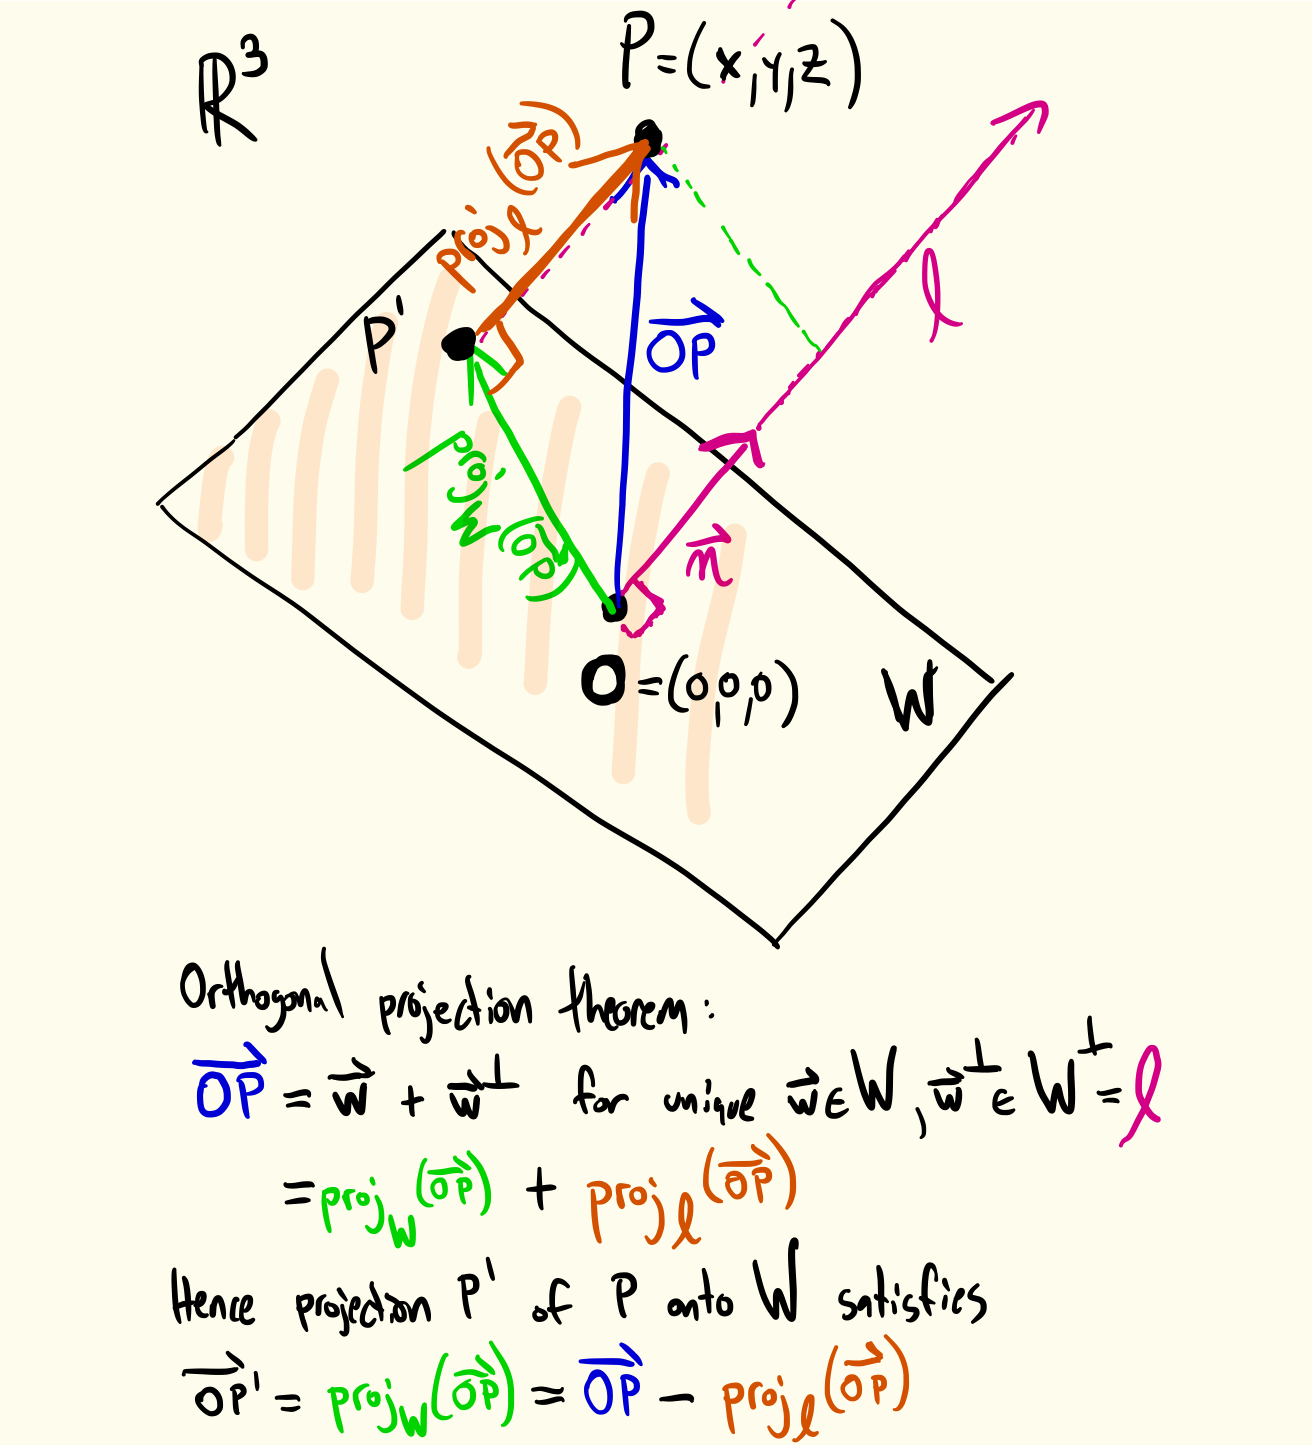
\includegraphics[width=3in]{Images/ProjPlaneDraw}
%\]
%\end{frame}
%\begin{frame}{Example}
%Define $\mathcal{P}: x+y+z=0$: i.e., $\boldn=(1,1,1)$. Let's use the first method in the previous slide to compute the projection of a point $P=(x,y,z)$ onto $\mathcal{P}$. 
%\bpause
%First pick \alert{any orthogonal} basis of $\mathcal{P}$: e.g., $B=\{(1,-1,0), (1,1,-2)\}$. 
%
%Then given $P=(x,y,z)$, the orthogonal projection formula yields 
%{\scriptsize
%\[
%\proj{(x,y,z)}{\mathcal{P}}=\frac{x-y}{2}(1,-1,0)+\frac{x+y-2z}{6}(1,1,-2). 
%\]
%}
%\pause We can express this in terms of matrix multiplication as 
%\[
%\proj{(x,y,z)}{\mathcal{P}}=\frac{1}{3}\begin{bmatrix}[rrr]
%2&-1&-1\\
%-1&2&-1\\
%-1&-1&2
%\end{bmatrix}
%\begin{bmatrix}
%x\\ y\\ z
%\end{bmatrix}.
%\]
%\pause
%\alert{Check}.  We get the same answer using the matrix formula from the previous slide, where we set $(a,b,c)=(1,1,1)$ !!
%\end{frame}
%\begin{frame}{General lines and planes in $\R^3$}
%So how do we proceed if have a line or plane in $\R^3$ that \alert{does not pass through the origin}? 
%\bb
%\pause
%\ii  Find any point $Q=(q_1,q_2,q_3)$ on the line/plane.
%\pause \ii Translate the whole picture by $-Q=(-q_1,-q_2, -q_3)$, which means we replace $P=(x,y,z)$ with $P-Q=(x-q_1,y-q_2,z-q_3)$.
%\pause \ii Apply our formulas from before, replacing $(x,y,z)$ with $(x-q_1,y-q_2,z-q_3)$
%\pause \ii Translate back by adding $Q$ to your answer. 
%\ee
%The result, as you can check, is as follows:
%\bpause
%\alert{Projection onto line}. If $\ell$ is the line passing through $Q=(q_1,q_2,q_3)$ with direction vector $(a,b,c)$, then 
%\[
%\proj{(x,y,z)}{\ell}=\frac{1}{a^2+b^2+c^2}\begin{bmatrix}
%a^2&ab&ac\\
%ab&b^2&bc\\
%ac&bc&c^2
%\end{bmatrix}
%\colvec{x-q_1\\ y-q_2\\ z-q_3}+\colvec{q_1\\ q_2\\ q_3}
%\]
%\bpause
%\alert{Projection onto plane}. If $\mathcal{P}$ is the plane passing through $Q=(q_1,q_2,q_3)$ with normal vector $\boldn=(a,b,c)$, then 
%\[
%\proj{(x,y,z)}{\mathcal{P}}=\frac{1}{a^2+b^2+c^2}\begin{bmatrix}
%b^2+c^2&-ab&-ac\\
%-ab&a^2+c^2&-bc\\
%-ac&-bc&a^2+b^2
%\end{bmatrix}
%\colvec{x-q_1\\ y-q_2\\ z-q_3}+
%\colvec{q_1\\ q_2\\ q_3}
%\]
%\end{frame}
%\begin{frame}{Example}
%\scriptsize
% Define $\mathcal{P}\colon (x-1)+(y-1)+2(z-1)=0$, and let $P=(0,1,5)$. Compute (a) $\proj{(0,1,5)}{\mathcal{P}}$, and (b) the distance from $P$ to $\mathcal{P}$.
%\bpause
%From the equation, we see that $\boldn=(1,1,2)$, and that $Q=(1,1,1)$ is a point in the plane. 
%\bpause
%Using the formula from the previous slide, we compute 
%\[
%\proj{(0,1,5)}{\mathcal{P}}=\frac{1}{6}\begin{bmatrix}
%5&-1&-2\\
%-1&5&-2\\
%-2&-2&2
%\end{bmatrix}
%\colvec{0-1\\ 1-1\\ 5-1\\}+
%\colvec{1\\ 1\\ 1}
%=\colvec{-7/6\\ -1/6 \\ 8/3}
%\]
%\pause
%By definition the distance between $(0,1,5)$ and $\mathcal{P}$ is 
%\[
%d((0,1,5), (-7/6, -1/6, 8/3))=\sqrt{49/36+49/36+49/9}=7\sqrt{6}/6.
%\]
%\pause
%Here is a picture of the situation. The distance from $P$ to $\mathcal{P}$ is the length of the pink normal line. 
%\[
%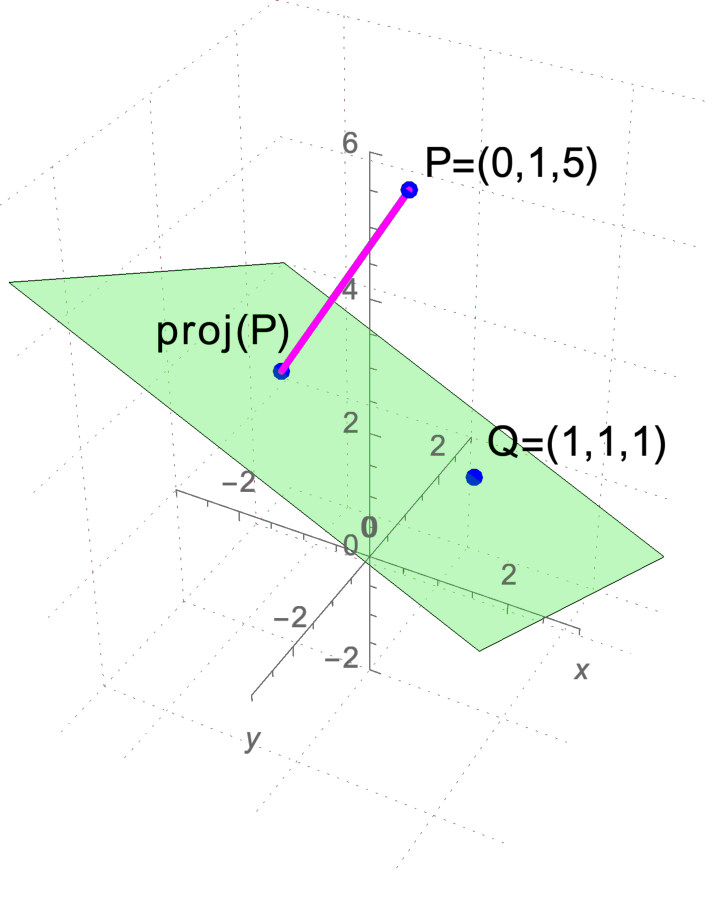
\includegraphics[width=1.5in]{Images/ProjPlane.pdf}
%\]
%
%\end{frame}
\begin{frame}{Example: sine/cosine series}
Let $V=C[0,2\pi]$ with inner product $\langle f, g\rangle=\int_0^{2\pi}f(x)g(x) \, dx$. 

We have seen that the set
\[
B=\{1, \cos(x),\sin(x),\cos(2x),\sin(2x), \dots , \cos(nx),\sin(nx)\} 
\] 
is orthogonal. Thus $B$ is an orthogonal basis of $W=\Span(B)$, which we might describe as the space of {\bf trigonometric polynomials of degree at most $n$}. 
\bpause
Given an arbitrary function $f(x)\in C[0,2\pi]$, its orthogonal projection onto $W$ is the function 
\[
\hat{f}(x)=a_0+a_1\cos(x)+b_1\sin(x)+a_2\cos(2x)+b_2\sin(2x)+\cdots +a_n\cos(nx)+b_n\sin(nx),
\]
where 
\[
a_0=\frac{1}{2\pi}\int_0^{2\pi} f(x) \ dx, \ a_j=\frac{1}{\pi}\int_0^{2\pi}f(x)\cos(jx)\, dx, \ b_k=\frac{1}{\pi}\int_0^{2\pi}f(x)\sin(kx)\, dx.
\]
\pause
The projection theorem tells us that $\hat{f}$ is the ``best" trigonometric polynomial approximation of $f(x)$ (of degree at most $n$), in the sense that for any other sinusoidal $g\in W$, $\left\vert\left\vert f-\hat{f}\right\vert\right\vert\leq \norm{f-g}$.  
\bpause 
This means in turn 
\[
\int_0^{2\pi} (f-\hat{f})^2\, dx\leq \int_0^{2\pi} (f-g)^2 \, dx.
\]
\end{frame}
\begin{frame}{Example: least-squares solution to $A\boldx=\boldy$}
Often in applications we have an $m\times n$  matrix $A$ and vector $\boldy\in\R^m$ for which the matrix equation 
\[
A\boldx=\boldy
\]  
has no solution. In terms of fundamental spaces, this means simply that $\boldy\notin \CS(A)$. Set $W=\CS(A)$.     
\bpause
In such situations we speak of a \alert{least-squares} solution to the matrix equation. This is a vector $\hat{\boldx}$ such that $A\hat{\boldx}=\hat{\boldy}$, where $\hat{\boldy}=\proj{\boldy}{W}$. Here the inner product is taken to be the dot product. 

Note: the equation $A\hat{\boldx}=\hat{\boldy}$ is guaranteed to have a solution since $\hat{\boldy}=\proj{\boldy}{W}$ lies in $\CS(A)$. 

\pause
The vector $\hat{\boldx}$ is called a least-square solutions because its image $\hat{\boldy}$ is the element of $\CS(A)$ that is ``closest" to $\boldy$ in terms of the dot product. 
\bspace 
Writing $\boldy=(y_1,y_2,\dots,y_n)$ and $\hat{\boldy}=(y_1',y_2',\dots, y_n')$, this means that $\hat{\boldy}$ minimizes the distance 
\[
\norm{\boldy-\hat{\boldy}}=\sqrt{(y_1-y_1')^2+(y_2-y_2')^2+\cdots +(y_n-y_n')^2}.
\]  
\end{frame}
\begin{frame}{Least-squares example (curve fitting)}
Suppose we wish to find an equation of a line $y=mx+b$ that best fits (in the least-square's sense) the following $(x,y)$ data points: $P_1=(-3,1), P_2=(1,2), P_3=(2,3)$. 

\pause
Then we seek $m$ and $b$ such that 
\begin{align*}
1&=m(-3)+b\\
2&=m(1)+b\\
3&=m(2)+b,
\end{align*} 
or equivalently, we wish to solve 
$
\begin{bmatrix}[rr]
-3&1\\ 1&1\\ 2&1
\end{bmatrix}
\begin{bmatrix}
m \\ b
\end{bmatrix}
=\begin{bmatrix}
1\\ 2\\ 3
\end{bmatrix}$. 
\bpause
This equation has no solution as $\boldy=(1,2,3)$ does no lie in $W=\CS(A)=\Span(\{(-3,1,2),(1,1,1)\}$. So instead we compute $\hat{\boldy}=\proj{\boldy}{W}=(13/14,33/14,38/14)$. (This was not hard to compute as conveniently the given basis of $W$ was already orthogonal!)  
\bpause
Finally we solve $A\begin{bmatrix}
m\\ b
\end{bmatrix}=\hat{\boldy}$, getting $m=5/14$, $b=28/14=2$. Thus $y=\frac{5}{14}x+2$ is the line best fitting the data in the least-squares sense. 
\end{frame}
\begin{frame}{Least-squares example contd.}
In what sense does $y=\frac{5}{14}x+2$ ``best" fit the data? 
\[
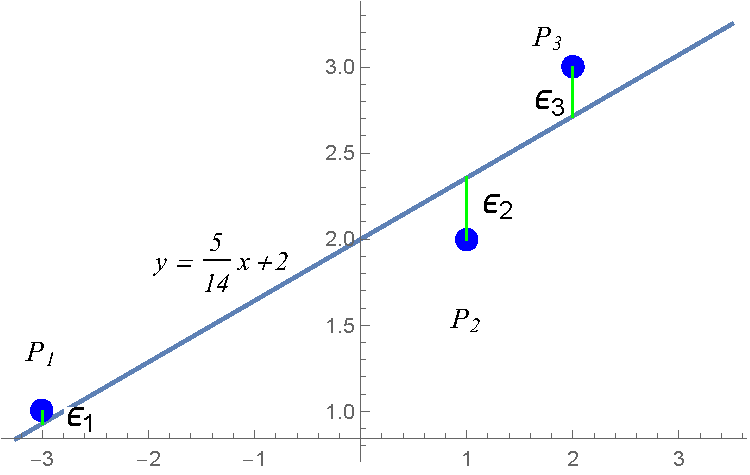
\includegraphics[width=2in]{Images/LeastSquares}
\]
Let $\boldy=(1,2,3)=(y_1,y_2,y_3)$ be the given $y$-values of the points, and $\hat{\boldy}=(y_1',y_2',y_3')$ be the projection we computed before. In the graph the values $\epsilon_i$ denote the vertical difference $\epsilon_i=y_i-y_i'$ between the data points, and our fitting line. 
\bpause 
The projection $\hat{\boldy}$ makes the error $\norm{\boldy-\hat{\boldy}}=\sqrt{  \epsilon_1^2+\epsilon_2^2+\epsilon_3^2}$ as small as possible. 

This means if I draw {\em any other line} and compute the corresponding differences $\epsilon_i'$ at the $x$-values -3, 1 and 2, then we have 
\[
\epsilon_1^2+\epsilon_2^2+\epsilon_3^2\leq (\epsilon_1')^2+(\epsilon_2')^2+(\epsilon_3')^2
\]  
\end{frame}
\begin{frame}{Finding least squares solutions}
As the last example illustrated, one method of finding a least-squares solution $\boldx$ to $A\boldx=\boldy$ is to 
first produce an orthogonal basis for $\CS(A)$, then compute $\hat{\boldy}=\proj{\boldy}{\CS(A)}$, and then use GE to solve $A\boldx=\hat{\boldy}$. 

\bpause
Alternatively, it turns out (through a little trickery) that $\hat{\boldy}=A\boldx$, where $\boldx$ is a solution to the equation 
\[
\boxed{A^TA\boldx=A^T\boldy}.
\]
This solves us the hassle of computing an orthogonal basis for $\CS(A)$; to find a least-squares solution $\boldx$ for $A\boldx=\boldy$, we simply use GE to solve the boxed equation. (Some more trickery shows a solution is guaranteed to exist!) 
\bpause
\alert{Example}. In the previous example we were seeking a least-squares solution $\boldx=\colvec{m\\ b}$ to $A\boldx=\boldy$, where 
$
A=\begin{bmatrix}[rr]
 -3&1\\
 1&1\\
 2&1
\end{bmatrix} , \boldy=\colvec{1\\2\\3}
$.

The equation $A^TA\boldx=A^T\boldy$ is thus 
\[
\begin{bmatrix}
14&0\\
0&3
\end{bmatrix}
\boldx=
\colvec{5\\ 6} 
\]
As you can see, $\boldx=\colvec{m\\ b}=\colvec{5/14\\ 2}$ is a least-squares solution, just as before
\end{frame}